\chapter{Introduzione}

	\section{Supervised vs Unsupervised}
		
		\begin{itemize}
			\item $\textbf{Supervised learning}$: È un approccio che è definito dall'uso di set di dati già etichettati: questi set di dati sono progettati per allenare (o "supervisionare") gli algoritmi nella classificazione dei dati o nella previsione accurata dei risultati.
				\\[1\baselineskip]
				Si parla di Supervised Learning quando è l'umano a fornire già delle etichette ai dati, in modo da dare una mano all'algoritmo nella sua fase di allenamento in quanto saprà già dall'inizio saprà quali sono i dati corretti.\\
				\\[1\baselineskip]
				L'apprendimento supervisionato può essere separato in due tipi di problemi durante il data mining: classificazione e regressione.
				\\[2\baselineskip]

			\item $\textbf{Unsupervised learning}$: Utilizza algoritmi di apprendimento automatico per analizzare e raggruppare set di dati non etichettati: questi algoritmi apprendono da soli i migliori pattern che rappresentano i dati, senza la necessità dell'intervento umano.
		\end{itemize}

	\clearpage

	\section{Regressione vs Classificazione}
		
		\begin{itemize}
			\item $\textbf{Regressione:}$ L'obiettivo principale dei problemi di regressione è quello di trovare una funzione ottimale che riesca a combinare alcune variabili $X$, dette anche $\textit{predittori}$, per produrre un valore in output, ovvero $Y$, il più preciso possibile.
				Alcuni esempi di problemi di regressione possono essere la stima dei prezzi di vendita di immobili oppure la stima della probabilità di un certo evento binario, come la probabilità di terremoti in certe regioni di un paese.
				\\[2\baselineskip]
			
			\item $\textbf{Classificazione:}$ L'altra categoria di problemi sono quelli di classificazione, ovvero problemi che richiedono di trovare una funzione che utilizza alcuni predittori $X$ per produrre in output un valore $Y$ discreto (può essere un'etichetta o una categoria).
			Un esempio di problema di classificazione può essere la categorizzazione di un sito come affidabile oppure non affidabile.
		\end{itemize}

	\clearpage

	\section{Train, Validation and Test}

		L'utilizzo di un algortimo per risolvere un certo problema prevede fondamentalmente due step: l'allenamento e la classificazione.
		È comune anche aggiungere la fase di validazione dopo la fase di allenamento, in cui è possibile, appunto, validare il modello$^{[1]}$ fornito dall'algoritmo.

			\subsection{Fase di Train}
			Il processo di allenamento dell'algoritmo consiste nel fornirgli un dataset su cui può imparare a classificare i dati (da qui il nome "Train Set") e costruire un modello ottimale sulla base di ciò che ha appreso.

			\subsection{Fase di Validation}
			Nella fase di Train, l'algoritmo impara le relazioni tra input $X$ e output $Y$.
			Per evitare di cadere nell'overfitting e avere una migliore capacità predittiva, viene dato al nostro modello dei dati che non ha mai visto e gli facciamo fare una predizione (anche questi dati devono essere già etichettati).
			\\[1\baselineskip]
			Dopo le predizioni su questi dati, verranno confrontati i risultati del modello (che denomineremo con $\hat{y}$) con le $y$ reali per vedere quanto il modello riesce a prevedere con una buona approssimazione la variabile target.
			Nel caso di performance scarse, bisogna aggiustare gli iperparametri del modello e ripartire dalla fase di train, finché il risultato ottenuto dalla fase di validation non sarà soddisfacente.
			
			\subsection{Fase di Test}
			Il processo di classificazione consiste nell'utilizzo del modello, precedentemente costruito nella fase di training, per predire le categorie o stimare i valori di nuovi dati.\\
			In questa fase viene fornito al modello un set di dati su cui valutare il modello; viene utilizzato solo dopo che il modello è stato completamente allenato.
			Il Test Set contiene dati accuratamente campionati che cercano di coprire le varie casistiche che il modello dovrà affrontare se utilizzato nel mondo reale.

		\begin{figure}[ht]
			\caption{Esempio di divisione del dataset}
			\centering
			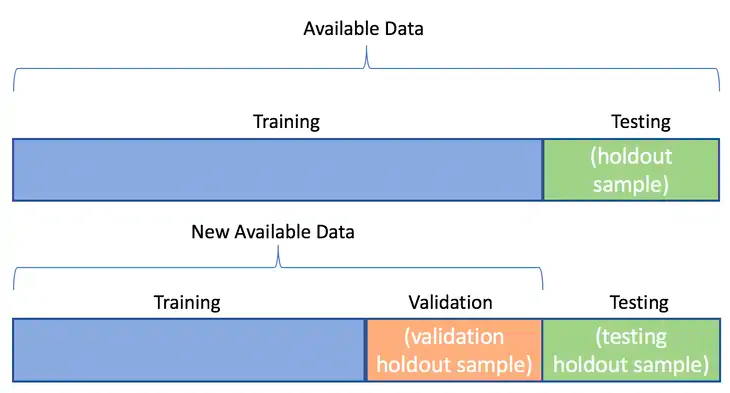
\includegraphics[width = 10cm, height = 4.2cm]{training-validation-test-split.png}
		\end{figure}

	\clearpage

	\section{Stratified Sampling}
		Il campionamento casuale generalmente va bene se il set di dati originale è sufficientemente grande proprio perché ogni sottoinsieme di $n$ istanze ha la stessa probabilità di essere selezionato come campione di qualsiasi altro sottoinsieme di $n$ istanze.
		\\
		Ma se il dataset non è sufficientemente grande, viene introdotta una distorsione a causa dell'errore di campionamento.
		\\[1\baselineskip]
		Il $\textbf{Stratified Sampling}$ è un metodo di campionamento che riduce l'errore di campionamento nei casi in cui la popolazione può essere suddivisa in sottogruppi:
		la popolazione viene divisa in sottogruppi omogenei, chamati $\textit{strati}$, per poi applicare il campionamento casuale semplice all'interno di ciascun sottogruppo.
		
		\begin{figure}[h]
			\caption{Esempio di Stratified Sampling}
			\centering
			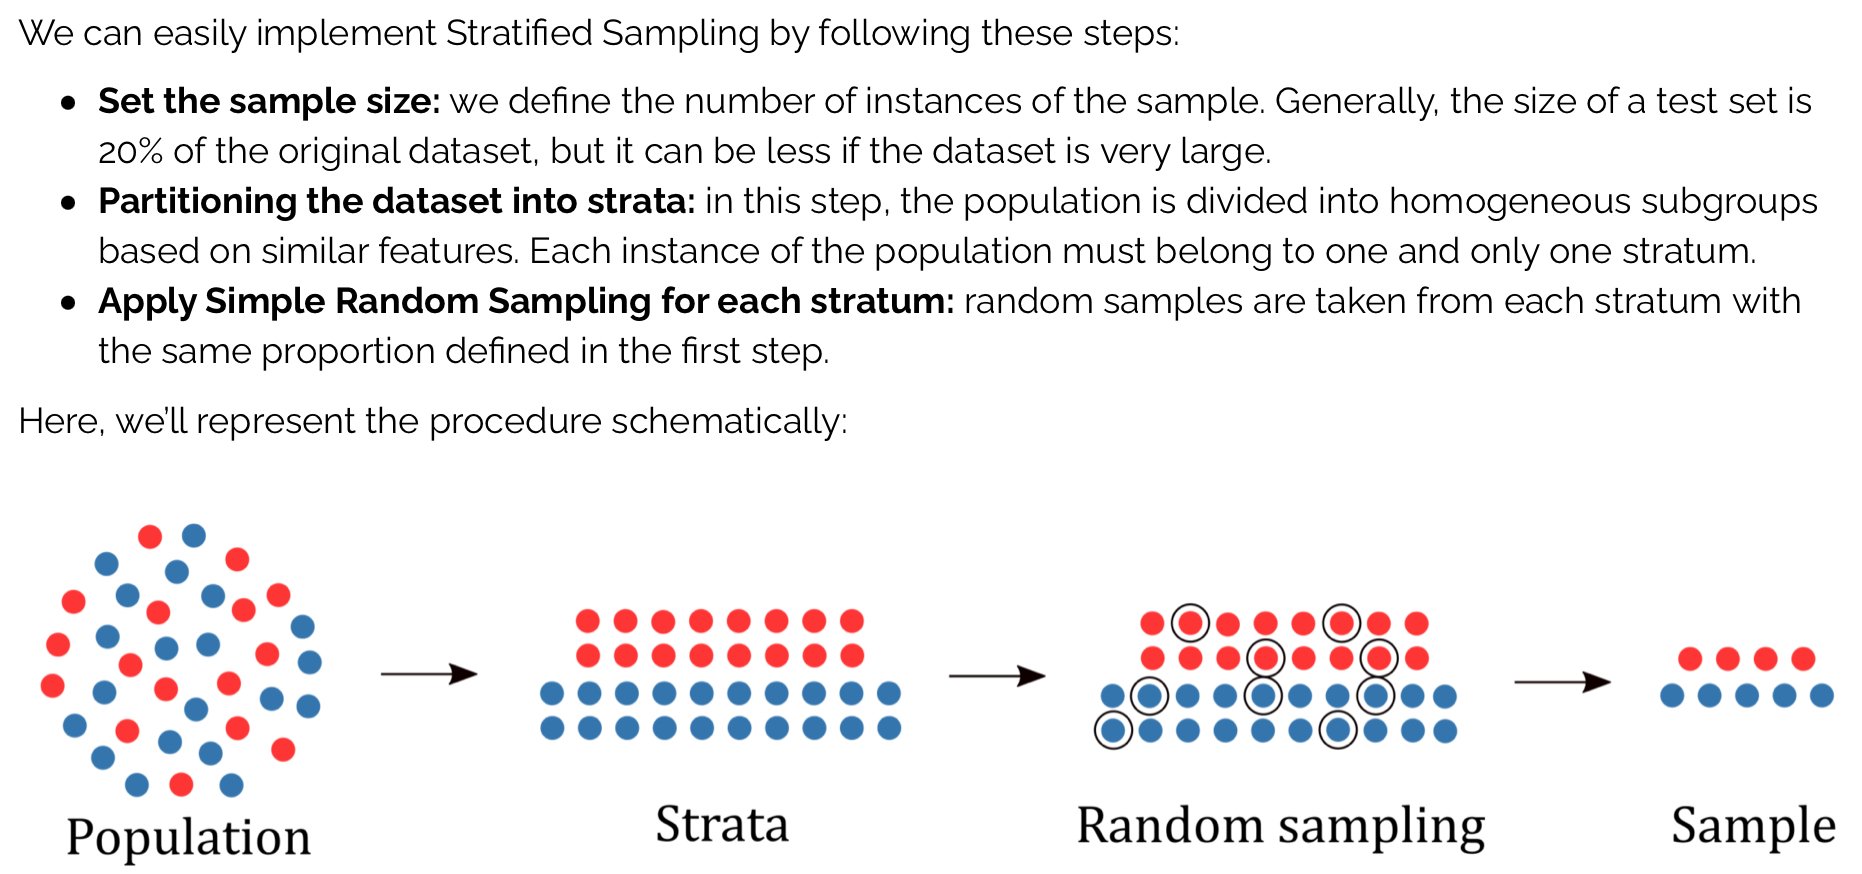
\includegraphics[width = 10cm, height = 4.2cm]{stratified-sampling-example.jpg}
		\end{figure}

	\clearpage

	\section{Cross-Validation}
		Il $\textbf{Cross-Validation}$ è una procedura di ricampionamento utilizzata per valutare i modelli di machine learning su un campione di dati limitato.
		La procedura ha un singolo parametro, ovvero $k$, che si riferisce al numero di gruppi in cui deve essere suddiviso un dato campione di dati.
		\\
		Pertanto, la procedura viene spesso chiamata
		\\
		$\textbf{K-Fold Cross-Validation}$.

		\subsubsection{Scelta di k}
			Il valore di $k$ deve essere scelto con cura per il campionamento di dati: un valore scelto in modo errato può risultare in una valutazione errata dell'abilità del modello.
			\\[1\baselineskip]
			Le tattiche più comuni per scegliere il valore di $k$ sono:

			\begin{itemize}
				\item $\textbf{Rappresentativo}$: il valore di k è scelto in modo tale che ciascun gruppo di campioni di dati train/test sia sufficientemente grande da essere statisticamente rappresentativo del set di dati più ampio;
				\item $\boldsymbol{k=10}$: il valore per $k$ è fissato a 10, un valore che è stato trovato attraverso la sperimentazione e che è risultato generalmente buono nella stima dell'abilità del modello;
				\item $\boldsymbol{k=n}$: il valore per $k$ è fissato a $n$, dove $n$ è la dimensione del dataset, per dare a ciascun campione l'opportunità di essere utilizzato nel validation set.
					\\
					Questo approccio è chiamato
					\\
					$\textbf{Leave-One-Out Cross-Validation}$ (LOOCV).
			\end{itemize}

		\begin{figure}[h]
			\caption{Esempio di Cross-Validation (k = 5)}
			\centering
			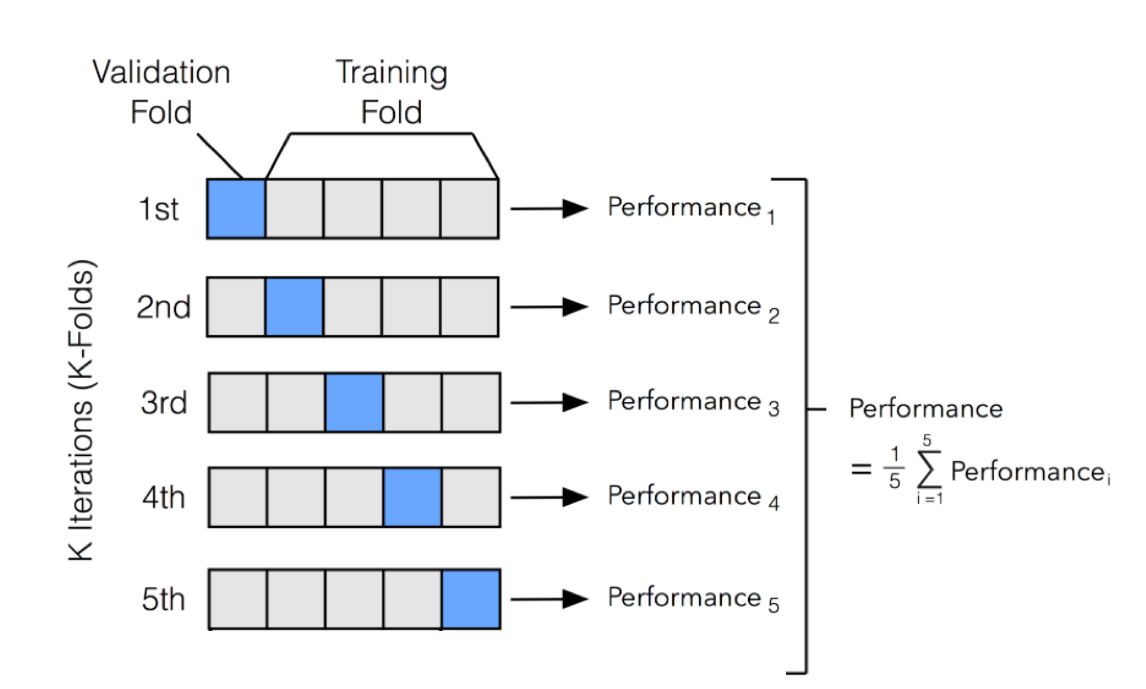
\includegraphics[width = 10cm]{CV-example.png}
		\end{figure}

	\clearpage

	\section{Underfitting vs Overfitting}
		L'overfitting e l'underfitting sono due problemi tipici in cui il modello raggiunge scarse performance nella classificazione dopo l'allenamento ma per motivi diversi.
			\begin{itemize}
				\item $\textbf{Underfitting}:$ ci sono pochi parametri nel modello e un'elevata discrepanza nella classificazione (Alto Bias).
				Il processo di apprendimento è troppo semplice.

				\item $\textbf{Overfitting}:$ ci sono troppi parametri nel modello e un'elevata variabilità della classificazione.
					Il modello è troppo complesso e sensibile ai dati di training (Alta Varianza).
			\end{itemize}

			\begin{figure}[h]
				\caption{Esempio di modello che sottostima}
				\centering
				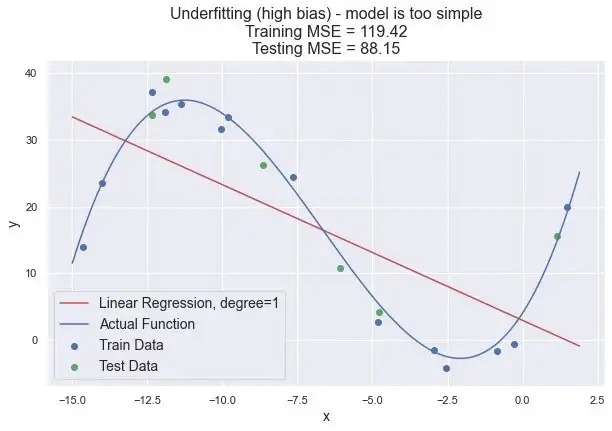
\includegraphics[width = 10cm]{underfitting.png}
			\end{figure}

			\begin{figure}[h]
				\caption{Esempio di modello che sovrastima}
				\centering
				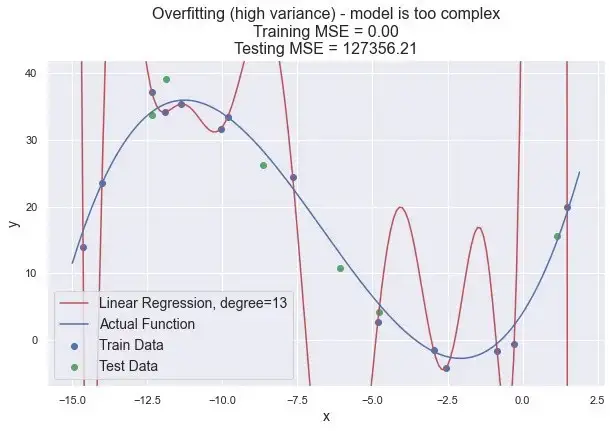
\includegraphics[width = 10cm]{overfitting.png}
			\end{figure}


			\begin{figure}[h]
				\caption{Esempio di modello buono, che non sovrastima o sottostima}
				\centering
				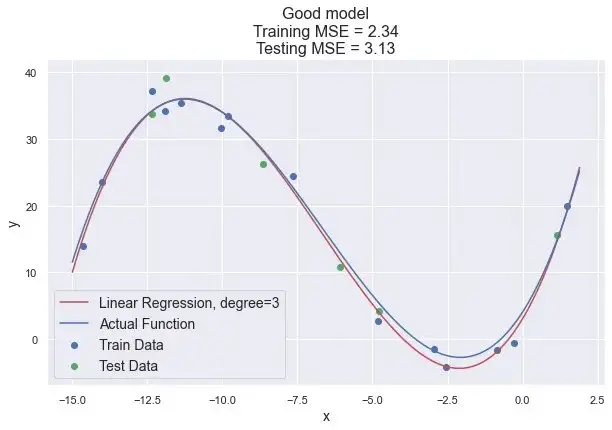
\includegraphics[width = 10cm]{good-model.png}
			\end{figure}

	\clearpage

	\section{ROC: Receiver Operating Characteristics}
		L'analisi delle $\textbf{Receiver Operating Characteristic}$ (ROC) è un approccio grafico per analizzare le prestazioni di un classificatore e studiarne l'output.
		\\[1\baselineskip]
		Utilizza una coppia di statistiche, tasso di Veri Positivi e tasso di Falsi Positivi.
		Le statistiche sono tracciate su un grafico bidimensionale, con tasso di falsi positivi sull'asse delle $x$ e tasso di veri positivi sull'asse delle $y$.
		\\[1\baselineskip]
		Poiché il classificatore può essere un valore arbitrario (output continuo), il confine tra le classi deve essere determinato da un valore di soglia oppure un'etichetta di classe discreta, che indica una delle classi.
		
		\begin{figure}[h]
			\caption[short]{Esempio di grafico ROC}
			\centering
			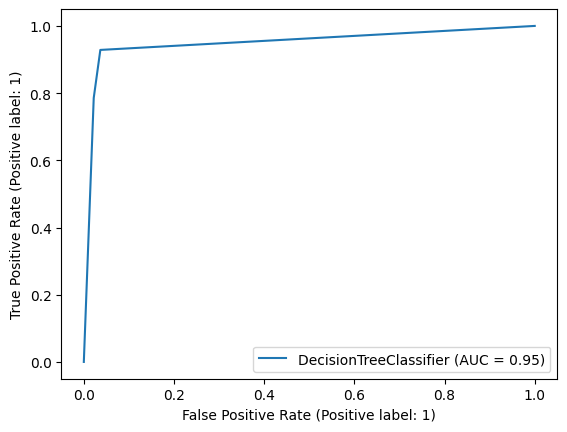
\includegraphics[width = 10cm]{roc-example.png}
		\end{figure}

		\begin{figure}[h]
			\caption[short]{Situazione ideale (1), situazione tipica (2) e situazione peggiore (non risce a discriminare) (3)}
			\centering
			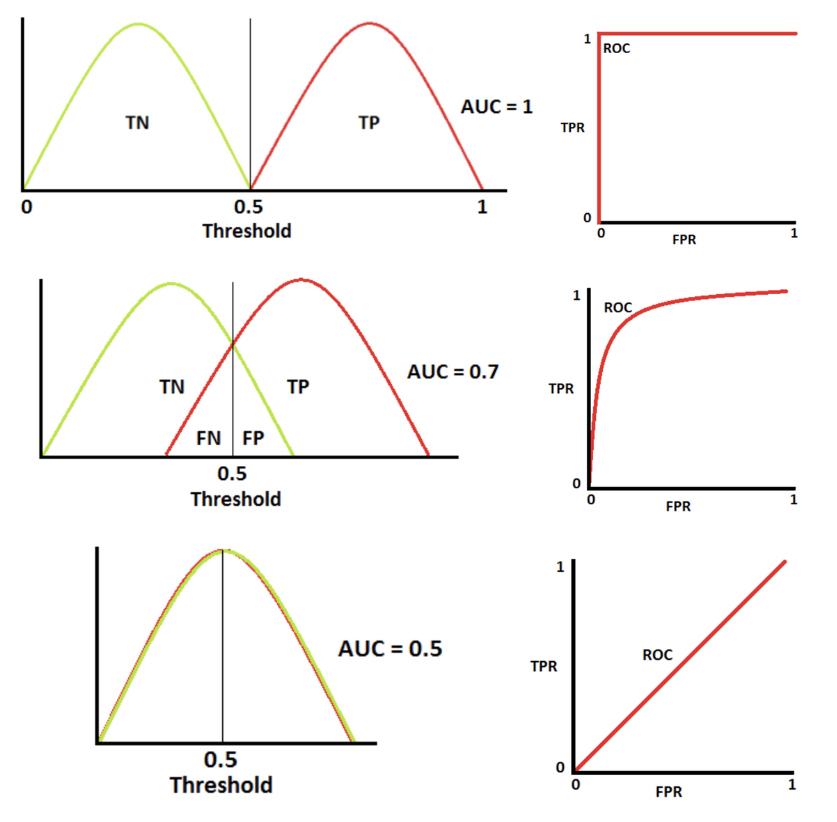
\includegraphics[width = 10cm]{roc-situations.png}
		\end{figure}

	\clearpage